% !TEX program = pdflatex
% Statistical Pharmacology via Kakutani Dichotomy I
% Companion computations: exp01_marginal_dki_criticality.py, paper01_compute_tables.py
\documentclass[11pt,reqno]{amsart}

\usepackage[T1]{fontenc}
\usepackage[utf8]{inputenc}
\usepackage{lmodern}
\usepackage[a4paper,margin=27mm]{geometry}
\usepackage{amsmath,amssymb,amsthm,mathtools}
\usepackage{booktabs}
\usepackage{graphicx}
\graphicspath{{./}{../figures/}}
\usepackage{array}
\usepackage{microtype}
\usepackage{enumitem}
\usepackage{xcolor}
\usepackage[colorlinks=true,linkcolor=blue!60!black,citecolor=blue!60!black,urlcolor=blue!60!black]{hyperref}

\theoremstyle{plain}
\newtheorem{theorem}{Theorem}[section]
\newtheorem{lemma}[theorem]{Lemma}
\newtheorem{proposition}[theorem]{Proposition}
\newtheorem{corollary}[theorem]{Corollary}
\theoremstyle{definition}
\newtheorem{definition}[theorem]{Definition}
\newtheorem{assumption}[theorem]{Assumption}
\theoremstyle{remark}
\newtheorem{remark}[theorem]{Remark}
\numberwithin{equation}{section}

\DeclareMathOperator{\Prob}{Prob}
\DeclareMathOperator{\Bern}{Bernoulli}
\newcommand{\dd}{\mathrm{d}}
\newcommand{\Dtail}{D_{\mathrm{tail}}}
\newcommand{\gEM}{\gamma_{\mathrm{EM}}}
\newcommand{\gnum}{\gamma_{\mathrm{num}}}
\newcommand{\gth}{\gamma_{\mathrm{th}}}
\newcommand{\gtail}{\gamma_{\mathrm{tail}}}
\newcommand{\geff}{\gamma_{\mathrm{eff}}}
\newcommand{\Rr}{\mathbb{R}}
\newcommand{\Nn}{\mathbb{N}}
\newcommand{\E}{\mathbb{E}}
\newcommand{\LA}{L_A}
\newcommand{\LB}{L_B}
\newcommand{\PA}{P_{A}}
\newcommand{\PB}{P_{B}}
\newcommand{\PAN}{P_{A,N}}
\newcommand{\PBN}{P_{B,N}}

\renewcommand{\abstractname}{Summary}

\title[Statistical pharmacology via Kakutani dichotomy I]{Statistical Pharmacology via Kakutani Dichotomy I:\\ The Marginal Drug Kakutani Index and the $\alpha_c=1/2$ Criticality Theorem in High-Dimensional Conformational Ensembles}

\author[Z. Chen]{Zhengyi Chen}
\address{Guangxi Key Laboratory of Drug Discovery and Optimization, School of Pharmacy, Guilin Medical University, Guilin 541199, P.~R. China}
\email{chenzhengyi@glmc.edu.cn}

\author[R. Chen]{Ruqing Chen}
\address{GUT Geoservice Inc., Montreal, Qu\'ebec, Canada}
\email{ruqing@hotmail.com}

\thanks{DOI: \href{https://doi.org/10.5281/zenodo.23005921}{10.5281/zenodo.23005921}. Sources, code and data: repository \texttt{kakutani-statistical-pharmacology-I} (see the Reproducibility paragraph of \S6).}
\thanks{This project was supported by the National Natural Science Foundation of China (No.~22464010), the Guangxi Natural Science Foundation of China (No.~2025GXNSFAA069294), and the 2025 Bagui Youth Top Talent Project.}
\date{27 September 2026}

\subjclass[2020]{Primary 60G30, 92C40; Secondary 62B10, 11M06, 46L30}
\keywords{Kakutani dichotomy, Hellinger distance, product measures, allostery, conformational ensembles, phase transitions, Euler--Maclaurin summation, finite-size scaling}

\begin{document}

\begin{abstract}
This is the first paper of a series that transports the central mechanism of \emph{Localized Bost--Connes systems} \cite{Chen2026}---a phase transition that is a tail event of an infinite product, invisible to every finite factor---from arithmetic thermodynamics to the statistical geometry of protein conformational ensembles. We model the conformational space of a protein with $N$ two-state local switches as $\Omega_N=\{0,1\}^N$ and two ligands $\LA,\LB$ as product measures $\PAN=\bigotimes_i\Bern(p_i)$, $\PBN=\bigotimes_i\Bern(q_i)$. We define the \emph{marginal drug Kakutani index} $K_N(\LA,\LB)=\sum_{i\le N}h_i$, the sum of the local squared Hellinger distances, the \emph{Kakutani affinity} $\Pi_N=\int_{\Omega_N}\sqrt{\dd\PAN\,\dd\PBN}=\prod_{i\le N}(1-h_i/2)$, and the \emph{doubling tail increment} $\Dtail(N)=K_{2N}-K_N$. We prove an exact quartic Taylor expansion of $h_i$ in the local shift $\delta_i=q_i-p_i$ (Lemma~\ref{lem:taylor}), whose odd cubic term vanishes identically at the maximal-entropy point $p=1/2$, where in fact $h(\delta)=2-\sqrt{1+2\delta}-\sqrt{1-2\delta}=\delta^2+\tfrac54\delta^4+\tfrac{21}{8}\delta^6+\cdots$ exactly. For the power-law allosteric decay model $q_i=p+c\,i^{-\alpha}$ with $p=1/2$, $c=1/10$, we prove the \emph{marginal drug Kakutani phase trichotomy} (Theorem~\ref{thm:trichotomy}): with $A=c^2/(4p(1-p))=10^{-2}$, one has $K_N\sim A N^{1-2\alpha}/(1-2\alpha)$ for $0<\alpha<1/2$, $K_N=A(\ln N+\gamma_{\mathrm{EM}})+C_\infty(1/2)+O(N^{-1})$ at $\alpha=1/2$, and $K_N\to K_\infty(\alpha)<\infty$ for $\alpha>1/2$; by Kakutani's theorem the infinite-dimensional ensembles are mutually singular in the first two regimes and equivalent in the third, so $\alpha_c=1/2$ is the unique critical exponent. At the critical point the doubling increment converges to the universal constant $A\ln2$ (Proposition~\ref{prop:doubling}). We then prove (Theorem~\ref{thm:fss}) that the effective exponent read from a finite regression window is $\geff(N;\alpha)=(1-2\alpha)/\bigl(1+(1-2\alpha)\zeta(2\alpha)N^{2\alpha-1}\bigr)$, so that the systematic upward bias observed near $\alpha_c$ is the simple pole of $\zeta$ at $2\alpha=1$ and not a numerical error, and that the doubling estimator cancels it identically (Corollary~\ref{cor:tail}). At $N=10^5$ the measured values $K_{10^5}=6.311486,\ 0.1211103,\ 0.0262136,\ 0.01658727$ for $\alpha=0.25,0.5,0.75,1$ agree with the Euler--Maclaurin predictions to relative accuracy $10^{-10}$ or better; the measured $\Dtail(10^5)|_{\alpha=1/2}=0.00693145$ agrees with $A\ln 2=0.00693147$ to $3.5\times10^{-6}$; and the anomalous regression exponent $\gnum(0.45)=0.1610$ is predicted analytically as $0.1601$ at the window centre and $0.1613$ on the window itself. The paper closes with an assessment and with the problem left to Paper~II: whether the off-diagonal covariance network of a correlated ensemble can drive the Kakutani transition on its own when every marginal is unchanged.
\end{abstract}

\maketitle
\tableofcontents

%%%%%%%%%%%%%%%%%%%%%%%%%%%%%%%%%%%%%%%%%%%%%%%%%%%%%%%%%%%%%%%%%%%%%%%%%%%%%%%
\section{Introduction: the binding affinity paradox and infinite-dimensional ensemble geometry}
\label{sec:intro}

\subsection*{The paradox}
Consider two ligands $\LA$ and $\LB$ bound to the same target---the presenilin-1 subunit of $\gamma$-secretase, or a class~A G-protein-coupled receptor---with macroscopically indistinguishable binding free energies,
\[
\Delta G_{\mathrm{bind}}(\LA)\approx\Delta G_{\mathrm{bind}}(\LB),
\]
and with local conformational footprints that are, residue by residue, almost identical: if $p_i$ and $q_i$ denote the probabilities that the $i$-th local switch (a side-chain rotamer, a backbone hydrogen bond, a water-mediated contact) is in its ``active'' state under $\LA$ and under $\LB$, then $\delta_i=q_i-p_i$ is small for every $i$, and for the distal residues it tends to zero. The paradox of allosteric drug design \cite{Nussinov2013,Motlagh2014} is that such a pair may nevertheless drive the protein into \emph{different}---in the extreme case, disjoint---downstream functional states: one ligand is a silent binder, the other a biased agonist or a $\gamma$-secretase modulator that shifts the A$\beta_{42}$/A$\beta_{40}$ ratio.

The classical thermodynamic description \cite{MWC1965} cannot resolve the paradox, because it aggregates the ensemble into a handful of global states whose populations are continuous functions of the $\delta_i$; if every $\delta_i$ is small, every population is nearly unchanged. The resolution proposed here is measure-theoretic. The object that governs downstream function is not any finite collection of marginals but the joint conformational law on the high-dimensional cube $\Omega_N=\prod_{i=1}^N\{0,1\}$, and for that law the question ``are $\PA$ and $\PB$ close?'' has, in the limit $N\to\infty$, only two possible answers.

\subsection*{The Kakutani dichotomy}
For infinite products of probability measures, Kakutani \cite{Kakutani1948} proved that $\bigotimes_i\mu_i$ and $\bigotimes_i\nu_i$ (with $\mu_i\sim\nu_i$ for each $i$) are either mutually absolutely continuous or mutually singular, according as $\sum_i\rho(\mu_i,\nu_i)$ converges or diverges, where $\rho$ is the squared Hellinger distance (equivalently, according as the product of the Hellinger affinities $\prod_i\int\sqrt{\dd\mu_i\,\dd\nu_i}$ is positive or zero). There is no third possibility, and the dichotomy is insensitive to any finite number of factors: the decision is made in the tail. The Gaussian analogue is the Feldman--H\'ajek theorem \cite{Feldman1958,Hajek1958}.

\begin{sloppypar}
This is precisely the structure that organises \cite{Chen2026}, the localized generalisation of the Bost--Connes system \cite{BostConnes1995}. There the $\mathrm{KMS}_\beta$ simplex of the $S$-local Bost--Connes system is $\Prob(G_S/\Xi_\beta^\perp)$, where the obstruction group
\end{sloppypar}
\[
\Xi_\beta(K,S)=\Bigl\{\chi\in\widehat{G_S}:\ \sum_{\mathfrak p\in S}N\mathfrak p^{-\beta}\,\bigl|1-\chi(\sigma_{\mathfrak p})\bigr|^2<\infty\Bigr\}
\]
is extracted from a Kakutani product criterion \cite[Ch.~1, Props.~3.3--3.4 and Thm.~3.6]{Chen2026}, and the central negative lesson of that book is that divergence of the partition function $\zeta_{K,S}(\beta)=\infty$ does \emph{not} imply uniqueness of the $\mathrm{KMS}_\beta$ state: the transition is ``a tail event---a Kakutani dichotomy in which every single factor is harmless, and only the infinite product degenerates'' \cite[Preface]{Chen2026}. The dictionary between that setting and the present one is given below; it is exact at the level of the criterion, and it is the reason we call the series \emph{statistical pharmacology via Kakutani dichotomy}.

\begin{center}\footnotesize
\textsc{The dictionary} between the localized Bost--Connes classification \cite{Chen2026} and the marginal drug Kakutani index.\\[4pt]
\begin{tabular}{@{}>{\raggedright\arraybackslash}p{0.17\textwidth}>{\raggedright\arraybackslash}p{0.38\textwidth}>{\raggedright\arraybackslash}p{0.38\textwidth}@{}}
\toprule
& Localized Bost--Connes system & Conformational ensemble \\
\midrule
Index set & primes $\mathfrak p\in S$ & local switches $i=1,\dots,N$ \\
Local weight & $N\mathfrak p^{-\beta}|1-\chi(\sigma_{\mathfrak p})|^2$ & $h_i$, the squared Hellinger distance of $\Bern(p_i)$, $\Bern(q_i)$ \\
Tail functional & $\sum_{\mathfrak p\in S}N\mathfrak p^{-\beta}|1-\chi(\sigma_{\mathfrak p})|^2$ & $K_N=\sum_{i\le N}h_i$ \\
Control parameter & inverse temperature $\beta$ & allosteric decay exponent $\alpha$ \\
Convergent regime & $\chi\in\Xi_\beta$, symmetry broken & $\PA\sim\PB$: localized perturbation \\
Divergent regime & $\chi\notin\Xi_\beta$, state unique & $\PA\perp\PB$: global allosteric re-shaping \\
False expectation & $\zeta_{K,S}(\beta)=\infty\Rightarrow$ uniqueness & $\delta_i\to0\Rightarrow\PA\approx\PB$ \\
\bottomrule
\end{tabular}
\end{center}

\subsection*{Main results}
Section~\ref{sec:dki} defines the product conformational ensemble, the marginal drug Kakutani index $K_N$, the Kakutani affinity $\Pi_N$ and the doubling tail increment $\Dtail(N)$, and proves the exact quartic expansion of the local Hellinger coordinate (Lemma~\ref{lem:taylor}); at $p=1/2$ the expansion is even and is given in closed form. Section~\ref{sec:trichotomy} proves the phase trichotomy at $\alpha_c=1/2$ for the power-law model $q_i=p+c\,i^{-\alpha}$ (Theorem~\ref{thm:trichotomy}), including the constants, and the universal doubling identity $\Dtail\to A\ln 2$ at criticality (Proposition~\ref{prop:doubling}). Section~\ref{sec:fss} develops the Euler--Maclaurin finite-size scaling theory: Theorem~\ref{thm:fss} gives the closed-form effective exponent $\geff(N;\alpha)$ and identifies the near-critical bias with the pole of $\zeta(2\alpha)$; Corollary~\ref{cor:tail} shows that the doubling estimator is unbiased. Section~\ref{sec:numerics} tabulates the numerical experiment of \texttt{exp01\_marginal\_dki\_criticality.py} (Tables~\ref{tab:bench} and~\ref{tab:scaling}, Figure~\ref{fig:phase}) against the analytic predictions. Section~\ref{sec:assessment} separates what has been established from what has not, and formulates the covariance problem for Paper~II.

\subsection*{Standing notation}
Throughout, $p\in(0,1)$ is the ground-state activation probability, $c\in(0,\min(p,1-p))$ the perturbation amplitude, $\alpha>0$ the decay exponent, and
\begin{equation}\label{eq:A}
A=A(p,c)=\frac{c^2}{4p(1-p)},\qquad H_N(s)=\sum_{i=1}^N i^{-s}\quad(s\in\Rr),\qquad \gamma_{\mathrm{EM}}=0.5772156649\ldots
\end{equation}
denote the prefactor, the generalised harmonic numbers and the Euler--Mascheroni constant. $\zeta$ is the Riemann zeta function, meromorphic on $\mathbb C$ with a simple pole at $1$ of residue $1$. In the numerical sections $p=1/2$, $c=1/10$, so $A=10^{-2}$.

%%%%%%%%%%%%%%%%%%%%%%%%%%%%%%%%%%%%%%%%%%%%%%%%%%%%%%%%%%%%%%%%%%%%%%%%%%%%%%%
\section{Product conformational spaces and the marginal drug Kakutani index}
\label{sec:dki}

\begin{definition}[Product conformational ensemble]\label{def:ensemble}
Let a protein carry $N$ local two-state conformational switches, and let $\Omega_N=\{0,1\}^N$ with coordinates $X=(X_1,\dots,X_N)$. Given activation profiles $(p_i)_{i\le N}$ and $(q_i)_{i\le N}$ in $(0,1)$ induced by ligands $\LA$ and $\LB$, the \emph{marginal (first-order) conformational ensembles} are the product measures
\begin{equation}\label{eq:product}
\PAN=\bigotimes_{i=1}^N\Bern(p_i),\qquad \PBN=\bigotimes_{i=1}^N\Bern(q_i),
\end{equation}
where $\Bern(r)$ is the law on $\{0,1\}$ with $\Bern(r)\{1\}=r$. For infinite profiles $(p_i)_{i\ge1}$, $(q_i)_{i\ge1}$ the same formulas with $N=\infty$ define $\PA$, $\PB$ on $\Omega_\infty=\{0,1\}^{\Nn}$ with the product $\sigma$-algebra.
\end{definition}

\begin{definition}[Local Hellinger coordinate, cumulative DKI, Kakutani affinity, doubling tail]\label{def:dki}
For $i\ge1$ let
\begin{equation}\label{eq:h}
h_i=h(p_i,q_i)=\bigl(\sqrt{p_i}-\sqrt{q_i}\bigr)^2+\bigl(\sqrt{1-p_i}-\sqrt{1-q_i}\bigr)^2
\end{equation}
be the squared Hellinger distance between $\Bern(p_i)$ and $\Bern(q_i)$. The \emph{marginal drug Kakutani index} (DKI), the \emph{Kakutani affinity}, and the \emph{doubling tail increment} are
\begin{equation}\label{eq:KPiD}
K_N(\LA,\LB)=\sum_{i=1}^N h_i,\qquad
\Pi_N(\LA,\LB)=\int_{\Omega_N}\sqrt{\dd\PAN\,\dd\PBN},\qquad
\Dtail(N)=K_{2N}-K_N .
\end{equation}
\end{definition}

\begin{lemma}[Exact quartic Taylor expansion of the local Hellinger distance]\label{lem:taylor}
Let $p\in(0,1)$ and $q=p+\delta$ with $|\delta|<\min(p,1-p)$. Then
\begin{equation}\label{eq:taylor}
h(p,p+\delta)=\frac{\delta^2}{4p(1-p)}\;-\;\frac{(1-2p)\,\delta^3}{8p^2(1-p)^2}\;+\;\frac{5\,(1-3p+3p^2)\,\delta^4}{64\,p^3(1-p)^3}\;+\;O(\delta^5),
\end{equation}
the series being convergent for $|\delta|<\min(p,1-p)$. In particular, at the maximal-entropy symmetric point $p=1/2$ the odd terms vanish identically, and in fact
\begin{equation}\label{eq:half}
h\bigl(\tfrac12,\tfrac12+\delta\bigr)=2-\sqrt{1+2\delta}-\sqrt{1-2\delta}=\sum_{k\ge1}a_k\,\delta^{2k},\qquad a_k=-2\binom{1/2}{2k}4^k>0,
\end{equation}
with $a_1=1$, $a_2=\tfrac54$, $a_3=\tfrac{21}{8}$, $a_4=\tfrac{429}{64}$, and the series converges for $|\delta|<1/2$. Thus
\begin{equation}\label{eq:half4}
h\bigl(\tfrac12,\tfrac12+\delta\bigr)=\delta^2+\tfrac54\delta^4+\tfrac{21}{8}\delta^6+O(\delta^8).
\end{equation}
\end{lemma}

\begin{proof}
Write $\sqrt{p+\delta}=\sqrt p\,(1+u)^{1/2}$ with $u=\delta/p$, $|u|<1$, and expand by the binomial series,
\[
(1+u)^{1/2}=1+\frac u2-\frac{u^2}8+\frac{u^3}{16}-\frac{5u^4}{128}+\frac{7u^5}{256}-\cdots,\qquad\binom{1/2}{n}=\frac{(-1)^{n-1}(2n-3)!!}{2^n\,n!}\ (n\ge1).
\]
Hence $\sqrt p-\sqrt{p+\delta}=-\sqrt p\,\bigl(\frac u2-\frac{u^2}8+\frac{u^3}{16}-\frac{5u^4}{128}+O(u^5)\bigr)$ and, squaring,
\begin{align*}
\bigl(\sqrt p-\sqrt{p+\delta}\bigr)^2
&=p\Bigl[\frac{u^2}{4}-2\cdot\frac u2\cdot\frac{u^2}{8}+\Bigl(\frac{u^4}{64}+2\cdot\frac u2\cdot\frac{u^3}{16}\Bigr)+O(u^5)\Bigr]\\
&=p\Bigl[\frac{u^2}{4}-\frac{u^3}{8}+\frac{5u^4}{64}+O(u^5)\Bigr]
=\frac{\delta^2}{4p}-\frac{\delta^3}{8p^2}+\frac{5\delta^4}{64p^3}+O(\delta^5).
\end{align*}
The second summand of \eqref{eq:h} is obtained from the first by the substitution $(p,\delta)\mapsto(1-p,-\delta)$:
\[
\bigl(\sqrt{1-p}-\sqrt{1-p-\delta}\bigr)^2=\frac{\delta^2}{4(1-p)}+\frac{\delta^3}{8(1-p)^2}+\frac{5\delta^4}{64(1-p)^3}+O(\delta^5).
\]
Adding, the quadratic coefficient is $\frac14\bigl(\frac1p+\frac1{1-p}\bigr)=\frac1{4p(1-p)}$; the cubic coefficient is
\[
\frac18\Bigl(\frac1{(1-p)^2}-\frac1{p^2}\Bigr)=\frac{p^2-(1-p)^2}{8p^2(1-p)^2}=\frac{2p-1}{8p^2(1-p)^2}=-\frac{1-2p}{8p^2(1-p)^2};
\]
and the quartic coefficient is
\[
\frac5{64}\Bigl(\frac1{p^3}+\frac1{(1-p)^3}\Bigr)=\frac{5\bigl((1-p)^3+p^3\bigr)}{64p^3(1-p)^3}=\frac{5(1-3p+3p^2)}{64p^3(1-p)^3},
\]
since $(1-p)^3+p^3=1-3p+3p^2$. This is \eqref{eq:taylor}; convergence follows from that of the two binomial series. At $p=1/2$ the cubic coefficient carries the factor $1-2p=0$. More generally, at $p=1/2$ the two summands of \eqref{eq:h} are exchanged by $\delta\mapsto-\delta$, so $h$ is an even function of $\delta$ and \emph{all} odd coefficients vanish. For the closed form, expand the squares in \eqref{eq:h}:
\begin{equation}\label{eq:hBC}
h(p,q)=(p+q)-2\sqrt{pq}+(2-p-q)-2\sqrt{(1-p)(1-q)}=2-2\Bigl(\sqrt{pq}+\sqrt{(1-p)(1-q)}\Bigr),
\end{equation}
and at $p=1/2$, $q=1/2+\delta$,
\[
2\sqrt{pq}=2\sqrt{\tfrac12\bigl(\tfrac12+\delta\bigr)}=\sqrt{1+2\delta},\qquad 2\sqrt{(1-p)(1-q)}=\sqrt{1-2\delta},
\]
whence $h=2-\sqrt{1+2\delta}-\sqrt{1-2\delta}$. With $x=2\delta$ and $\sqrt{1\pm x}=\sum_n\binom{1/2}{n}(\pm x)^n$, the odd powers cancel and $h=-2\sum_{k\ge1}\binom{1/2}{2k}x^{2k}=\sum_{k\ge1}\bigl(-2\binom{1/2}{2k}4^k\bigr)\delta^{2k}$. Since $\binom{1/2}{2k}<0$ for $k\ge1$, all $a_k>0$; the values $a_1=-2\cdot(-\frac18)\cdot4=1$, $a_2=-2\cdot(-\frac5{128})\cdot16=\frac54$, $a_3=-2\cdot(-\frac{21}{1024})\cdot64=\frac{21}8$, $a_4=-2\cdot(-\frac{429}{32768})\cdot256=\frac{429}{64}$ follow from $\binom{1/2}{2}=-\frac18$, $\binom{1/2}{4}=-\frac5{128}$, $\binom{1/2}{6}=-\frac{21}{1024}$, $\binom{1/2}{8}=-\frac{429}{32768}$. Consistency with \eqref{eq:taylor} at $p=1/2$: $\frac{5(1-\frac32+\frac34)}{64\cdot\frac1{64}}=\frac54$.
\end{proof}

\begin{remark}[Fisher information and the quality of the quadratic term]\label{rem:fisher}
The quadratic coefficient $1/(4p(1-p))$ is one quarter of the Fisher information $I(p)=1/(p(1-p))$ of the Bernoulli family, in accordance with the general identity $h(P_\theta,P_{\theta+\delta})=\frac14 I(\theta)\delta^2+O(\delta^3)$ \cite{LeCam1986}. At $p=1/2$ the absence of the cubic term makes the quadratic approximation accurate to fourth order: the relative quartic correction at the largest shift $\delta_1=c=1/10$ is $a_2c^2=\frac54\times10^{-2}=1.25\%$, and the exact value is $h(\frac12,\frac6{10})=2-\sqrt{1.2}-\sqrt{0.8}=0.0101276940\ldots$, against $\delta^2=0.01$ and $\delta^2+\frac54\delta^4=0.010125$. For $i\ge2$ the shift is smaller and the correction is smaller still ($a_2c^2i^{-2\alpha}$). Since all $a_k>0$, the function $\delta\mapsto h(\frac12,\frac12+\delta)/\delta^2$ is increasing in $|\delta|$, so for the model of Section~\ref{sec:trichotomy} we have the two-sided bound
\begin{equation}\label{eq:sandwich}
\delta_i^2\le h_i\le(1+\varepsilon_c)\,\delta_i^2,\qquad \varepsilon_c:=\frac{h(\frac12,\frac12+c)}{c^2}-1=0.0127694\ldots\quad(c=\tfrac1{10}),
\end{equation}
which is what the qualitative part of the trichotomy needs.
\end{remark}

\begin{lemma}[Product formula for the affinity]\label{lem:affinity}
For every $N$,
\begin{equation}\label{eq:affinity}
\Pi_N=\prod_{i=1}^N\Bigl(\sqrt{p_iq_i}+\sqrt{(1-p_i)(1-q_i)}\Bigr)=\prod_{i=1}^N\Bigl(1-\frac{h_i}{2}\Bigr),
\end{equation}
and $0<1-h_i/2\le1$ with equality iff $p_i=q_i$. Moreover
\begin{equation}\label{eq:logPi}
\ln\Pi_N=-\frac{K_N}{2}-Q_N,\qquad 0\le Q_N\le\frac14\sum_{i=1}^N h_i^2 .
\end{equation}
\end{lemma}

\begin{proof}
On the finite set $\Omega_N$ the integral $\int\sqrt{\dd\PAN\,\dd\PBN}$ is the sum over $x\in\Omega_N$ of $\sqrt{\PAN\{x\}\PBN\{x\}}$. Since $\PAN\{x\}=\prod_i p_i^{x_i}(1-p_i)^{1-x_i}$ and likewise for $\PBN$, the square root factorises and the sum over $x$ factorises into $\prod_i\bigl(\sqrt{p_iq_i}+\sqrt{(1-p_i)(1-q_i)}\bigr)$. By the identity \eqref{eq:hBC} from the proof of Lemma~\ref{lem:taylor}, $\sqrt{p_iq_i}+\sqrt{(1-p_i)(1-q_i)}=1-h_i/2$, which is the second equality in \eqref{eq:affinity}. By Cauchy--Schwarz, $\sqrt{p_iq_i}+\sqrt{(1-p_i)(1-q_i)}\le\sqrt{(p_i+1-p_i)(q_i+1-q_i)}=1$ with equality iff $(\sqrt{p_i},\sqrt{1-p_i})$ and $(\sqrt{q_i},\sqrt{1-q_i})$ are proportional, i.e.\ iff $p_i=q_i$; positivity is clear. For \eqref{eq:logPi} put $x_i=h_i/2\in(0,1/2]$ (indeed $h_i<2$ because $\sqrt{p_iq_i}>0$). The series $-\ln(1-x)=\sum_{m\ge1}x^m/m$ gives $-\ln(1-x)-x=\sum_{m\ge2}x^m/m\in\bigl[0,\,x^2\sum_{m\ge0}2^{-m}/2\bigr]=[0,x^2]$ for $0\le x\le1/2$. Summing over $i$ with $Q_N:=\sum_i\bigl(-\ln(1-x_i)-x_i\bigr)$ yields \eqref{eq:logPi}.
\end{proof}

\begin{theorem}[Kakutani]\label{thm:kakutani}
Let $(p_i),(q_i)\subset(0,1)$ and $\PA,\PB$ be as in Definition~\ref{def:ensemble}. Then exactly one of the following holds:
\begin{enumerate}[label=\textup{(\roman*)}]
\item $\sum_{i\ge1}h_i<\infty$; then $\Pi_\infty:=\lim_N\Pi_N>0$ and $\PA\sim\PB$ (mutually absolutely continuous);
\item $\sum_{i\ge1}h_i=\infty$; then $\Pi_\infty=0$ and $\PA\perp\PB$ (mutually singular).
\end{enumerate}
\end{theorem}

\begin{proof}
This is Kakutani's theorem \cite{Kakutani1948} for the factors $\mu_i=\Bern(p_i)$, $\nu_i=\Bern(q_i)$, which are equivalent since $p_i,q_i\in(0,1)$; the criterion there is $\prod_i\int\sqrt{\dd\mu_i\dd\nu_i}>0$ versus $=0$, and by Lemma~\ref{lem:affinity} $\prod_i(1-h_i/2)>0$ iff $\sum_ih_i<\infty$ (because $0<h_i/2\le1/2$ and $\ln(1-x)\asymp-x$ on $[0,1/2]$).
\end{proof}

%%%%%%%%%%%%%%%%%%%%%%%%%%%%%%%%%%%%%%%%%%%%%%%%%%%%%%%%%%%%%%%%%%%%%%%%%%%%%%%
\section{The marginal drug Kakutani phase trichotomy at \texorpdfstring{$\alpha_c=1/2$}{alpha\_c=1/2}}
\label{sec:trichotomy}

\subsection*{Standing assumption: power-law allosteric decay}
Throughout this section and the next, $p_i=p=\tfrac12$ for all $i$, and $q_i=p+c\,i^{-\alpha}$ with $c=\tfrac1{10}$ and $\alpha>0$. Thus $\delta_i=c\,i^{-\alpha}\in(0,c]$, all $q_i\in(\tfrac12,\tfrac35]$, and $A=c^2/(4p(1-p))=c^2=10^{-2}$. With $a_k$ the coefficients of \eqref{eq:half} we write
\begin{equation}\label{eq:RC}
R_N(\alpha):=\sum_{k\ge2}a_k\,c^{2k}\,H_N(2k\alpha),\qquad C_\infty(\alpha):=\sum_{k\ge2}a_k\,c^{2k}\,\zeta(2k\alpha)\quad(\alpha>\tfrac14)
\end{equation}
for the higher-order Hellinger corrections; Lemma~\ref{lem:series} shows that $C_\infty(\alpha)=\lim_NR_N(\alpha)$. We state the two main results of the section first; their proofs follow the two lemmas.

\begin{theorem}[Marginal drug Kakutani phase trichotomy]\label{thm:trichotomy}
Under the standing assumption, with $A=10^{-2}$ and $R_N(\alpha)$, $C_\infty(\alpha)$ as in \eqref{eq:RC}, the following hold as $N\to\infty$.
\begin{enumerate}[label=\textup{(\arabic*)}]
\item \textbf{Supercritical allosteric phase, $0<\alpha<\tfrac12$.}
\begin{equation}\label{eq:super}
K_N(\alpha)=\frac{A}{1-2\alpha}\,N^{1-2\alpha}+A\,\zeta(2\alpha)+\frac A2N^{-2\alpha}+R_N(\alpha)+O(N^{-2\alpha-1})\ \longrightarrow\ \infty,
\end{equation}
where $R_N(\alpha)=C_\infty(\alpha)+O(N^{1-4\alpha})$ if $\alpha>\frac14$ and $R_N(\alpha)=O(N^{1-4\alpha})$ (resp.\ $O(\ln N)$) if $\alpha<\frac14$ (resp.\ $=\frac14$). Consequently $\ln\Pi_N=-\frac12K_N(\alpha)+O(1)$ for $\alpha>\frac14$ and $\ln\Pi_N=-\frac12K_N(\alpha)\bigl(1+o(1)\bigr)$ in general; $\Pi_N\to0$ and $\PA\perp\PB$.
\item \textbf{Critical Kakutani boundary, $\alpha=\alpha_c=\tfrac12$.}
\begin{equation}\label{eq:crit}
\begin{gathered}
K_N(\tfrac12)=A\Bigl(\ln N+\gamma_{\mathrm{EM}}+\frac1{2N}\Bigr)+C_\infty(\tfrac12)+O\bigl(c^4N^{-1}\bigr)\ \longrightarrow\ \infty,\\
C_\infty(\tfrac12)=\sum_{k\ge2}a_kc^{2k}\zeta(k)=2.0885\times10^{-4},
\end{gathered}
\end{equation}
and
\begin{equation}\label{eq:critPi}
\Pi_N=\kappa\,N^{-A/2}\bigl(1+O(N^{-1})\bigr),\qquad \kappa=\exp\Bigl(-\tfrac12\bigl(A\gamma_{\mathrm{EM}}+C_\infty(\tfrac12)\bigr)-Q_\infty\Bigr)\in(0,1),
\end{equation}
so $\Pi_N\to0$ by a critical power-law collapse and $\PA\perp\PB$.
\item \textbf{Subcritical localized phase, $\alpha>\tfrac12$.}
\begin{equation}\label{eq:sub}
\begin{gathered}
K_\infty(\alpha):=\lim_{N\to\infty}K_N(\alpha)=A\,\zeta(2\alpha)+C_\infty(\alpha)<\infty,\\
K_N(\alpha)=K_\infty(\alpha)-A\,\zeta(2\alpha,N+1)-O\bigl(c^4N^{1-4\alpha}\bigr),
\end{gathered}
\end{equation}
with $A\zeta(2\alpha,N+1)=\frac{A}{2\alpha-1}N^{1-2\alpha}\bigl(1+O(N^{-1})\bigr)$; $\Pi_\infty(\alpha)=\lim_N\Pi_N>0$ and $\PA\sim\PB$.
\end{enumerate}
In particular $\alpha_c=\tfrac12$ is the unique critical exponent: the infinite-dimensional ensembles are mutually singular for $\alpha\le\frac12$ and equivalent for $\alpha>\frac12$.
\end{theorem}

\begin{proposition}[Scale-invariant doubling tail identity at $\alpha_c=1/2$]\label{prop:doubling}
Under the standing assumption at $\alpha=\tfrac12$,
\begin{equation}\label{eq:doubling}
\begin{gathered}
\Dtail(N)=K_{2N}-K_N=A\ln2-\frac{A}{4N}+O\bigl(c^4N^{-1}\bigr)+O(N^{-2}),\\
\lim_{N\to\infty}\Dtail(N)=A\ln2=0.0069314718\ldots
\end{gathered}
\end{equation}
The limit is independent of $N$ and of the Euler--Mascheroni and $C_\infty$ constants, which cancel identically.
\end{proposition}

We first record the Euler--Maclaurin expansion of the generalised harmonic numbers, with the constant identified.

\begin{lemma}[Euler--Maclaurin expansion of $H_N(s)$]\label{lem:EM}
For $s>0$, $s\ne1$, as $N\to\infty$,
\begin{equation}\label{eq:EMs}
H_N(s)=\frac{N^{1-s}}{1-s}+\zeta(s)+\frac{N^{-s}}{2}-\frac{s\,N^{-s-1}}{12}+O(N^{-s-3}),
\end{equation}
and for $s=1$,
\begin{equation}\label{eq:EM1}
H_N(1)=\ln N+\gamma_{\mathrm{EM}}+\frac1{2N}-\frac1{12N^2}+O(N^{-4}).
\end{equation}
For $s>1$ one has the exact tail identity $\zeta(s)-H_N(s)=\sum_{i>N}i^{-s}=\zeta(s,N+1)$ (Hurwitz zeta), and $\frac{(N+1)^{1-s}}{s-1}\le\zeta(s,N+1)\le\frac{N^{1-s}}{s-1}$.
\end{lemma}

\begin{proof}
Apply the Euler--Maclaurin summation formula \cite{Apostol1999} to $f(x)=x^{-s}$ on $[1,N]$ with two Bernoulli terms:
\begin{gather*}
\sum_{i=1}^N f(i)=\int_1^N f(x)\,\dd x+\frac{f(1)+f(N)}2+\frac{B_2}{2!}\bigl(f'(N)-f'(1)\bigr)+R_2(N),\\
R_2(N)=-\int_1^N\frac{\overline B_3(x)}{3!}f'''(x)\,\dd x,
\end{gather*}
where $B_2=\frac16$, $\overline B_3$ is the periodic Bernoulli function, and the remainder can be pushed to any order. Since $f'''(x)=-s(s+1)(s+2)x^{-s-3}$ is absolutely integrable at $\infty$ for $s>0$, $R_2(N)=R_2(\infty)+O(N^{-s-2})$, and pushing one more step, $R_2(N)=R_2(\infty)+\frac{B_4}{4!}f'''(N)+O(N^{-s-4})$ with $B_4=-\frac1{30}$, which is $O(N^{-s-3})$. For $s\ne1$, $\int_1^Nx^{-s}\dd x=\frac{N^{1-s}-1}{1-s}$ and $f'(N)=-sN^{-s-1}$, so
\begin{gather*}
H_N(s)=\frac{N^{1-s}}{1-s}+C(s)+\frac{N^{-s}}2-\frac{s N^{-s-1}}{12}+O(N^{-s-3}),\\
C(s):=-\frac1{1-s}+\frac12+\frac s{12}+R_2(\infty).
\end{gather*}
For $s>1$ the term $N^{1-s}/(1-s)\to0$, so $C(s)=\lim_NH_N(s)=\zeta(s)$. The function $C(s)$ defined by the displayed formula is analytic in $\operatorname{Re}s>-2$, $s\ne1$ (the remainder integral converges there), and $C(s)=\zeta(s)$ for $s>1$; by analytic continuation $C(s)=\zeta(s)$ for all $s>0$, $s\ne1$ \cite[\S2.1, eq.~(2.1.4)]{Titchmarsh1986}. This is \eqref{eq:EMs}. For $s=1$ the same computation with $\int_1^Nx^{-1}\dd x=\ln N$ gives $H_N(1)=\ln N+C(1)+\frac1{2N}-\frac1{12N^2}+O(N^{-4})$, and $C(1)=\lim_N(H_N(1)-\ln N)=\gamma_{\mathrm{EM}}$ by definition of the Euler--Mascheroni constant. The tail identity for $s>1$ is the definition of the Hurwitz zeta function, and the bracketing bounds follow from comparing $\sum_{i>N}i^{-s}$ with $\int_N^\infty x^{-s}\dd x$ and $\int_{N+1}^\infty x^{-s}\dd x$, the summand being decreasing.
\end{proof}

\begin{lemma}[Series representation of the DKI]\label{lem:series}
Under the standing assumption, for every $N\ge1$,
\begin{equation}\label{eq:Kseries}
K_N(\alpha)=\sum_{k\ge1}a_k\,c^{2k}\,H_N(2k\alpha)=A\,H_N(2\alpha)+R_N(\alpha),
\end{equation}
with $a_k$ as in \eqref{eq:half} and $R_N(\alpha)$ as in \eqref{eq:RC}, the double series converging absolutely. Moreover $0<R_N(\alpha)\le\varepsilon_c\,A\,H_N(4\alpha)$, so that
\begin{equation}\label{eq:Rbound}
R_N(\alpha)=
\begin{cases}
O(1), & \alpha>\tfrac14,\\
O(\ln N), & \alpha=\tfrac14,\\
O(N^{1-4\alpha}), & \alpha<\tfrac14 .
\end{cases}
\end{equation}
In every case $R_N(\alpha)=o\bigl(N^{1-2\alpha}\bigr)$ when $\alpha<\tfrac12$, and for $\alpha>\tfrac14$
\begin{equation}\label{eq:Cinf}
\lim_{N\to\infty}R_N(\alpha)=\sum_{k\ge2}a_k\,c^{2k}\,\zeta(2k\alpha)=C_\infty(\alpha),
\end{equation}
with $R_N(\alpha)=C_\infty(\alpha)-a_2c^4\zeta(4\alpha,N+1)-\cdots=C_\infty(\alpha)+O(N^{1-4\alpha})$.
\end{lemma}

\begin{proof}
By Lemma~\ref{lem:taylor}, $h_i=\sum_ka_k\delta_i^{2k}=\sum_ka_kc^{2k}i^{-2k\alpha}$, with all terms positive and $\delta_i\le c<\frac12$; summing over $i\le N$ and interchanging the finite sum with the convergent positive series gives \eqref{eq:Kseries}. For the bound, $R_N=\sum_i(h_i-\delta_i^2)$ and, since all $a_k>0$ and $\delta_i\le c$, $h_i-\delta_i^2=\delta_i^4\sum_{k\ge2}a_k\delta_i^{2k-4}\le\delta_i^4\sum_{k\ge2}a_kc^{2k-4}=\delta_i^4\,\bigl(h(\tfrac12,\tfrac12+c)-c^2\bigr)/c^4=\varepsilon_c\,\delta_i^4/c^2$, whence $R_N\le\varepsilon_c c^{-2}\sum_i c^4i^{-4\alpha}=\varepsilon_cAH_N(4\alpha)$. The growth statements \eqref{eq:Rbound} are Lemma~\ref{lem:EM} applied to $H_N(4\alpha)$, and $N^{1-4\alpha}=o(N^{1-2\alpha})$, $\ln N=o(N^{1/2})$. For $\alpha>1/4$ each $H_N(2k\alpha)$ with $k\ge2$ increases to $\zeta(2k\alpha)<\infty$ and dominated convergence (dominating series $\sum_ka_kc^{2k}\zeta(2k\alpha)\le\sum_ka_kc^{2k}\zeta(4\alpha)<\infty$) gives \eqref{eq:Cinf}; the rate follows from the tail identity of Lemma~\ref{lem:EM} applied termwise, the $k=2$ term dominating.
\end{proof}

\begin{proof}[Proof of Theorem~\ref{thm:trichotomy}]
\emph{Qualitative part.} By \eqref{eq:sandwich}, $A\,H_N(2\alpha)\le K_N(\alpha)\le(1+\varepsilon_c)A\,H_N(2\alpha)$, and $H_N(2\alpha)$ converges iff $2\alpha>1$. Hence $\sum_ih_i<\infty$ iff $\alpha>\frac12$, and Theorem~\ref{thm:kakutani} gives $\PA\sim\PB$ for $\alpha>\frac12$ and $\PA\perp\PB$ for $\alpha\le\frac12$, together with $\Pi_\infty>0$ resp.\ $\Pi_\infty=0$.

\emph{(1).} Insert \eqref{eq:EMs} with $s=2\alpha\in(0,1)$ into $K_N=AH_N(2\alpha)+R_N$ (Lemma~\ref{lem:series}); the term $-\frac{A s}{12}N^{-s-1}$ is absorbed into $O(N^{-2\alpha-1})$. The description of $R_N$ is \eqref{eq:Rbound}--\eqref{eq:Cinf}. For $\Pi_N$ use \eqref{eq:logPi}: $Q_N\le\frac14\sum_ih_i^2\le\frac14(1+\varepsilon_c)^2c^4H_N(4\alpha)$, which is bounded for $\alpha>\frac14$ and $O(N^{1-4\alpha})=o(N^{1-2\alpha})$ otherwise.

\emph{(2).} At $\alpha=\frac12$ the $k$-th term of \eqref{eq:Kseries} is $a_kc^{2k}H_N(k)$. For $k=1$ use \eqref{eq:EM1}: $AH_N(1)=A(\ln N+\gamma_{\mathrm{EM}}+\frac1{2N})+O(N^{-2})$. For $k\ge2$, $H_N(k)=\zeta(k)-\zeta(k,N+1)$ with $0<\zeta(k,N+1)\le N^{1-k}/(k-1)\le N^{-1}$, so $\sum_{k\ge2}a_kc^{2k}H_N(k)=C_\infty(\frac12)-\theta_N$, $0<\theta_N\le N^{-1}\sum_{k\ge2}a_kc^{2k}=\varepsilon_cAN^{-1}$; this is the $O(c^4N^{-1})$ term. The numerical value of $C_\infty(\frac12)$ is computed from $a_2c^4\zeta(2)=1.25\times10^{-4}\times1.6449341=2.05617\times10^{-4}$, $a_3c^6\zeta(3)=2.625\times10^{-6}\times1.2020569=3.1554\times10^{-6}$, $a_4c^8\zeta(4)=6.7031\times10^{-8}\times1.0823232=7.255\times10^{-8}$, and $a_5c^{10}\zeta(5)=1.97\times10^{-9}$, the remaining terms being below $10^{-10}$: $C_\infty(\frac12)=2.08847\times10^{-4}$. For \eqref{eq:critPi}, by \eqref{eq:logPi}, $\ln\Pi_N=-\frac12K_N-Q_N$ with $Q_N$ increasing to $Q_\infty\le\frac14(1+\varepsilon_c)^2c^4\zeta(2)=4.22\times10^{-5}$ and $Q_\infty-Q_N\le\frac14(1+\varepsilon_c)^2c^4\zeta(2,N+1)=O(N^{-1})$; inserting \eqref{eq:crit} gives $\ln\Pi_N=-\frac A2\ln N-\frac12(A\gamma_{\mathrm{EM}}+C_\infty(\frac12))-Q_\infty+O(N^{-1})$.

\emph{(3).} For $\alpha>\frac12$ every $H_N(2k\alpha)$ increases to $\zeta(2k\alpha)$, and the limit \eqref{eq:sub} follows from monotone convergence in \eqref{eq:Kseries}. The finite-$N$ correction is
\[
K_\infty-K_N=A\,\zeta(2\alpha,N+1)+\sum_{k\ge2}a_kc^{2k}\,\zeta(2k\alpha,N+1);
\]
by the tail bounds of Lemma~\ref{lem:EM} the $k$-th term is at most $a_kc^{2k}N^{1-2k\alpha}/(2k\alpha-1)$, and the sum over $k\ge2$ is $O(c^4N^{1-4\alpha})$. The stated form of $A\zeta(2\alpha,N+1)$ is \eqref{eq:EMs} for $s=2\alpha>1$ combined with the tail identity.
\end{proof}

\begin{remark}[Numerical confirmation of the constants at $N=10^5$]\label{rem:constants}
The analytic expressions of Theorem~\ref{thm:trichotomy} reproduce the measured values of Table~\ref{tab:bench} digit by digit.
\begin{itemize}[leftmargin=*]
\item \emph{Critical point.} $A(\ln10^5+\gamma_{\mathrm{EM}}+\tfrac1{2\cdot10^5})=10^{-2}\times(11.51292546+0.57721566+0.00000500)=0.1209014613$. Adding $C_\infty(\frac12)=0.0002088470$ gives $0.1211103083$; the measured value is $K_{10^5}(\frac12)=0.1211103068$, the difference $1.5\times10^{-9}$ being the $-\theta_N=O(c^4N^{-1})$ truncation of the $k\ge2$ terms. The leading logarithm accounts for $99.83\%$ of the value; the quartic Hellinger correction $a_2c^4\zeta(2)$ for $0.17\%$; everything beyond that for $3\times10^{-6}$ relative.
\item \emph{$\alpha=0.75$.} $A\zeta(1.5)=10^{-2}\times2.6123753=0.0261237535$ and $C_\infty(0.75)=a_2c^4\zeta(3)+a_3c^6\zeta(4.5)+\cdots=1.50257\times10^{-4}+2.769\times10^{-6}+6.8\times10^{-8}=1.53095\times10^{-4}$, so $K_\infty(0.75)=0.0262768494$. The truncation $A\zeta(1.5,10^5+1)=6.32454\times10^{-5}$ (its leading form $2AN^{-1/2}=6.32456\times10^{-5}$) gives $K_{10^5}(0.75)=0.0262136040$; measured: $0.0262136040$.
\item \emph{$\alpha=1$.} $A\zeta(2)=10^{-2}\times\pi^2/6=0.0164493407$, $C_\infty(1)=a_2c^4\zeta(4)+a_3c^6\zeta(6)+a_4c^8\zeta(8)+\cdots=1.35290\times10^{-4}+2.6705\times10^{-6}+6.73\times10^{-8}=1.38030\times10^{-4}$, so $K_\infty(1)=0.0165873709$; the truncation $A\zeta(2,10^5+1)=9.99995\times10^{-8}\approx A/N$ gives $K_{10^5}(1)=0.0165872709$; measured: $0.0165872709$.
\item \emph{$\alpha=0.25$.} $A\bigl(2\sqrt N+\zeta(\frac12)+\frac1{2\sqrt N}\bigr)=10^{-2}\times(632.4555320-1.4603545+0.0015811)=6.3099676$; here $R_N(\frac14)=a_2c^4H_N(1)+a_3c^6H_N(\frac32)+\cdots=1.25\times10^{-4}\times12.0901461+2.625\times10^{-6}\times2.6060+\cdots=0.0015182$ is logarithmically growing, in accordance with \eqref{eq:Rbound}; the total $6.3114858$ matches the measured $6.3114858$.
\end{itemize}
\end{remark}

\begin{proof}[Proof of Proposition~\ref{prop:doubling}]
By \eqref{eq:crit} applied at $2N$ and at $N$,
\begin{align*}
K_{2N}-K_N&=A\Bigl(\ln2N-\ln N+\frac1{4N}-\frac1{2N}\Bigr)+\bigl(C_\infty(\tfrac12)-C_\infty(\tfrac12)\bigr)+O(c^4N^{-1})+O(N^{-2})\\
&=A\ln2-\frac A{4N}+O(c^4N^{-1})+O(N^{-2}),
\end{align*}
where the $O(N^{-2})$ collects the $-\frac1{12N^2}$ terms of \eqref{eq:EM1}. The $O(c^4N^{-1})$ term is $\theta_N-\theta_{2N}$, which is at most $\varepsilon_cAN^{-1}=1.3\times10^{-4}\,A/N$ in absolute value and is therefore numerically dominated by $-A/(4N)$.
\end{proof}

\begin{remark}
Table~\ref{tab:bench} gives $\Dtail(10^5)|_{\alpha=1/2}=0.0069314474$; the prediction $A\ln2-A/(4N)=0.0069314718-0.0000000250=0.0069314468$ is off by $6\times10^{-10}$, i.e.\ the $\theta$-terms, and the relative deviation from the universal limit $A\ln2$ is $3.5\times10^{-6}$. Reading down the $\alpha=0.5$ block of Table~\ref{tab:bench}, $\Dtail(N)$ increases monotonically to $A\ln 2$ from below, exactly as the sign of $-A/(4N)$ dictates.
\end{remark}

%%%%%%%%%%%%%%%%%%%%%%%%%%%%%%%%%%%%%%%%%%%%%%%%%%%%%%%%%%%%%%%%%%%%%%%%%%%%%%%
\section{Euler--Maclaurin finite-size scaling theory and resolution of the near-critical anomaly}
\label{sec:fss}

The numerical experiment estimates the exponent of $K_N$ by ordinary least squares of $\ln K_N$ on $\ln N$ over a log-uniform grid in the window $[10^3,10^5]$ (sixty points), and reports $\gnum(\alpha)$ against the asymptotic value $\gth=1-2\alpha$. Table~\ref{tab:scaling} shows that the agreement is excellent for $\alpha\le0.25$ and degrades steadily as $\alpha\uparrow\frac12$, the discrepancy reaching $0.061$ at $\alpha=0.45$. We now prove that this is the signature of the pole of $\zeta(s)$ at $s=1$ and not a defect of the computation.

\begin{theorem}[Analytic mechanism of the finite-size logarithmic slope bias near $\alpha_c=1/2$]\label{thm:fss}
Let $0<\alpha<\frac12$ and let $\widetilde K_N(\alpha)=A\bigl[\frac{N^{1-2\alpha}}{1-2\alpha}+\zeta(2\alpha)\bigr]$ be the two-term Euler--Maclaurin form of $K_N(\alpha)$ from \eqref{eq:super}. Define the effective (local logarithmic) exponent $\geff(N;\alpha)=\dd\ln\widetilde K_N/\dd\ln N$. Then
\begin{equation}\label{eq:geff}
\geff(N;\alpha)=\frac{1-2\alpha}{1+(1-2\alpha)\,\zeta(2\alpha)\,N^{2\alpha-1}},
\end{equation}
and:
\begin{enumerate}[label=\textup{(\roman*)}]
\item $\geff(N;\alpha)>1-2\alpha$ for every finite $N$ (upward bias), and $\geff(N;\alpha)\downarrow1-2\alpha$ as $N\to\infty$ at the rate $N^{2\alpha-1}$;
\item the bias diverges relative to $1-2\alpha$ as $\alpha\uparrow\frac12$: with $\epsilon=1-2\alpha\to0^+$, $(1-2\alpha)\zeta(2\alpha)N^{2\alpha-1}=-1+\epsilon(\ln N+\gamma_{\mathrm{EM}})+O(\epsilon^2)$, and hence
\begin{equation}\label{eq:geffcrit}
\lim_{\alpha\uparrow1/2}\geff(N;\alpha)=\frac1{\ln N+\gamma_{\mathrm{EM}}},
\end{equation}
which is the exact local exponent of the critical law $A(\ln N+\gamma_{\mathrm{EM}})$: the effective exponent is continuous across $\alpha_c$, whereas $\gth=1-2\alpha$ jumps from $0^+$ to the logarithmic regime;
\item the true DKI satisfies $\dd\ln K_N/\dd\ln N=\geff(N;\alpha)\bigl(1+O(N^{-1})+O(c^2N^{-2\alpha})\bigr)$ where $\dd/\dd\ln N$ acts on the Euler--Maclaurin expansion, so \eqref{eq:geff} is the leading finite-size law for the regression exponent.
\end{enumerate}
\end{theorem}

\begin{corollary}[Constant cancellation via the doubling tail estimator]\label{cor:tail}
Under the standing assumption of \S\ref{sec:trichotomy} with $0<\alpha<\frac12$,
\begin{equation}\label{eq:Dtailsuper}
\Dtail(N)=A\,\frac{2^{1-2\alpha}-1}{1-2\alpha}\,N^{1-2\alpha}\Bigl(1+O(N^{-1})+O\bigl(c^2N^{-2\alpha}\bigr)\Bigr),
\end{equation}
the constants $A\zeta(2\alpha)$ and $C_\infty(\alpha)$ cancelling identically. Consequently
\begin{equation}\label{eq:gtail}
\gtail(N;\alpha):=\frac{\dd\ln\Dtail(N)}{\dd\ln N}=1-2\alpha+O(N^{-1})+O\bigl(c^2N^{-2\alpha}\bigr),
\end{equation}
and the log-log regression of $\Dtail$ recovers the true exponent without the pole-induced bias of Theorem~\ref{thm:fss}, uniformly in $\alpha$ up to the critical point.
\end{corollary}

The proofs rest on one elementary fact about $\zeta$.

\begin{lemma}[Sign and pole of $\zeta$ on $(0,1)$]\label{lem:zetaneg}
For $0<s<1$, $\zeta(s)<0$. As $s\uparrow1$, $\zeta(s)=\frac1{s-1}+\gamma_{\mathrm{EM}}+O(s-1)$; in particular $(1-s)\zeta(s)\to-1$.
\end{lemma}

\begin{proof}
For $s>0$ the Dirichlet eta function $\eta(s)=\sum_{n\ge1}(-1)^{n-1}n^{-s}$ converges (alternating series with terms decreasing to $0$) and is positive, being a sum of the positive pairs $(2m-1)^{-s}-(2m)^{-s}$. For $s>1$, $\eta(s)=(1-2^{1-s})\zeta(s)$ by splitting $\zeta$ into even and odd $n$, and the identity persists for $s>0$, $s\ne1$, by analytic continuation. For $0<s<1$ the factor $1-2^{1-s}$ is negative, hence $\zeta(s)=\eta(s)/(1-2^{1-s})<0$. The Laurent expansion at $s=1$ is classical \cite[\S2.1]{Titchmarsh1986}: $\zeta(s)-\frac1{s-1}$ is entire and equals $\gamma_{\mathrm{EM}}$ at $s=1$ (this is also \eqref{eq:EM1} read against \eqref{eq:EMs} as $s\to1$).
\end{proof}

\begin{proof}[Proof of Theorem~\ref{thm:fss}]
Differentiating $\ln\widetilde K_N$ with respect to $\ln N$, using $\dd N^{1-2\alpha}/\dd\ln N=(1-2\alpha)N^{1-2\alpha}$,
\[
\geff=\frac{A\,N^{1-2\alpha}}{A\bigl[\frac{N^{1-2\alpha}}{1-2\alpha}+\zeta(2\alpha)\bigr]}
=\frac{(1-2\alpha)N^{1-2\alpha}}{N^{1-2\alpha}+(1-2\alpha)\zeta(2\alpha)}
=\frac{1-2\alpha}{1+(1-2\alpha)\zeta(2\alpha)N^{2\alpha-1}},
\]
which is \eqref{eq:geff}. (i): by Lemma~\ref{lem:zetaneg}, $\zeta(2\alpha)<0$ and $1-2\alpha>0$, so the denominator is $<1$; it is positive as soon as $N^{1-2\alpha}>(1-2\alpha)|\zeta(2\alpha)|$, which holds throughout the window considered (at $\alpha=0.45$, $N=10^3$: $N^{0.1}=1.995>0.943$); $N^{2\alpha-1}\to0$ gives the limit and the rate. (ii): put $s=2\alpha=1-\epsilon$. By Lemma~\ref{lem:zetaneg}, $\epsilon\,\zeta(1-\epsilon)=-1+\gamma_{\mathrm{EM}}\epsilon+O(\epsilon^2)$, and $N^{-\epsilon}=1-\epsilon\ln N+O(\epsilon^2)$; multiplying, $\epsilon\zeta(1-\epsilon)N^{-\epsilon}=-1+\epsilon(\ln N+\gamma_{\mathrm{EM}})+O(\epsilon^2)$, so the denominator of \eqref{eq:geff} is $\epsilon(\ln N+\gamma_{\mathrm{EM}})+O(\epsilon^2)$ and $\geff=\epsilon/\bigl(\epsilon(\ln N+\gamma_{\mathrm{EM}})+O(\epsilon^2)\bigr)\to1/(\ln N+\gamma_{\mathrm{EM}})$. That this is the local exponent of $A(\ln N+\gamma_{\mathrm{EM}})$ is the computation $\dd\ln(\ln N+\gamma_{\mathrm{EM}})/\dd\ln N=1/(\ln N+\gamma_{\mathrm{EM}})$. (iii): the terms of \eqref{eq:super} omitted from $\widetilde K_N$ are $\frac A2N^{-2\alpha}$, of relative size $N^{-1}$ against the leading term, and $R_N(\alpha)-C_\infty(\alpha)$ resp.\ $R_N(\alpha)$, of relative size $O(c^2N^{-2\alpha})$ by Lemma~\ref{lem:series} ($R_N\le\varepsilon_cAH_N(4\alpha)$ against $AN^{1-2\alpha}/(1-2\alpha)$); the constant $C_\infty(\alpha)$, when present, adds to $A\zeta(2\alpha)$ and shifts the constant in \eqref{eq:geff} by the relative amount $C_\infty/(A\zeta(2\alpha))=O(c^2)$, which is within the same error class. Differentiating the expansion term by term (it is an asymptotic expansion in powers of $N$, so differentiation with respect to $\ln N$ is legitimate) gives the claim.
\end{proof}

\begin{remark}[The $\alpha=0.45$ anomaly, resolved]\label{rem:045}
At $\alpha=0.45$, $2\alpha=0.9$ and $\zeta(0.9)=-9.4301140\ldots$ (from $\zeta(s)=\frac1{s-1}+\gamma_{\mathrm{EM}}-\gamma_1(s-1)+\cdots$ with $\gamma_1=-0.0728158$: $-10+0.5772157-0.0072816=-9.4300659$, the remaining Stieltjes terms contributing $-4.8\times10^{-5}$). At the logarithmic centre $N_*=10^4$ of the regression window $[10^3,10^5]$, $N_*^{2\alpha-1}=10^{-0.4}=0.3981072$, so the denominator of \eqref{eq:geff} is $1+0.1\times(-9.4301140)\times0.3981072=1-0.3754185=0.6245815$ and
\[
\geff(10^4;0.45)=\frac{0.1000}{0.6245815}=0.16011 .
\]
The regression value is $\gnum(0.45)=0.16103$. The residual $0.0009$ is the difference between the local exponent at the window centre and the least-squares slope over the whole window: fitting $\ln\widetilde K_N$ on the same sixty-point grid gives $\gEM^{\mathrm{fit}}(0.45)=0.1613$ (Table~\ref{tab:scaling}), within $3\times10^{-4}$ of $\gnum$. The same formula predicts the full column: $0.9001$, $0.8003$, $0.7007$, $0.6016$, $0.5037$, $0.4080$, $0.3167$, $0.2327$, $0.1601$ against the measured $0.8995$, $0.7998$, $0.7004$, $0.6016$, $0.5039$, $0.4085$, $0.3174$, $0.2336$, $0.1610$. The anomaly is therefore entirely accounted for by the negative, pole-dominated constant $A\zeta(2\alpha)$ competing with the slowly growing $AN^{1-2\alpha}/(1-2\alpha)$ inside a finite window. Note also the sanity check of \eqref{eq:geffcrit}: at $N=10^4$ the critical local exponent is $1/(9.2103+0.5772)=0.1022$, so the sequence $\geff(10^4;\alpha)$ decreases continuously through $0.1601$ at $\alpha=0.45$ to $0.1022$ at $\alpha=\frac12$, while $1-2\alpha$ is already $0.1$ at $\alpha=0.45$ and $0$ at $\alpha_c$.
\end{remark}

\begin{proof}[Proof of Corollary~\ref{cor:tail}]
Apply \eqref{eq:super} at $2N$ and $N$ and subtract. The $N$-independent terms $A\zeta(2\alpha)$ and, for $\alpha>\frac14$, $C_\infty(\alpha)$ cancel exactly; the power terms give $\frac A{1-2\alpha}\bigl((2N)^{1-2\alpha}-N^{1-2\alpha}\bigr)=A\frac{2^{1-2\alpha}-1}{1-2\alpha}N^{1-2\alpha}$; the Euler--Maclaurin term $\frac A2\bigl((2N)^{-2\alpha}-N^{-2\alpha}\bigr)$ is $O(N^{-2\alpha})$, i.e.\ relative $O(N^{-1})$; and the difference of the $R$-terms is, by Lemma~\ref{lem:series}, at most $\varepsilon_cA\bigl(H_{2N}(4\alpha)-H_N(4\alpha)\bigr)\le\varepsilon_cAN\cdot N^{-4\alpha}=O(c^2\cdot AN^{1-2\alpha}\cdot N^{-2\alpha})$, i.e.\ relative $O(c^2N^{-2\alpha})$. Taking logarithms and differentiating the asymptotic expansion gives \eqref{eq:gtail}.
\end{proof}

\begin{remark}
The last column of Table~\ref{tab:scaling} confirms the corollary: $\gtail$ agrees with $1-2\alpha$ to within $5\times10^{-4}$ at every $\alpha$, including $\gtail(0.45)=0.1001$ where the direct estimator gives $0.1610$. The small residuals at small $\alpha$ ($0.8995$ against $0.9$) are the $O(c^2N^{-2\alpha})$ term, which is largest when $\alpha$ is smallest ($c^2N^{-0.1}\approx4\times10^{-3}$ at $N=10^4$). At the critical point itself the same estimator gives the universal constant of Proposition~\ref{prop:doubling}.
\end{remark}

\begin{remark}[The critical slope]
For $\alpha=\frac12$ the experiment regresses $K_N$ on $\ln N$ over the same window and obtains the slope $0.0099992$, against $A=0.01$ predicted by \eqref{eq:crit}. The deficit $8\times10^{-7}$ is the derivative $-A/(2N)$ of the Euler--Maclaurin term $A/(2N)$, which is $-5\times10^{-6}$ at the left end of the window and is averaged down by the log-uniform weights; it is of the size predicted and of the predicted sign.
\end{remark}

%%%%%%%%%%%%%%%%%%%%%%%%%%%%%%%%%%%%%%%%%%%%%%%%%%%%%%%%%%%%%%%%%%%%%%%%%%%%%%%
\section{Numerical verification tables and phase diagram analysis}
\label{sec:numerics}

\subsection*{Protocol}
\begin{sloppypar}
The script \texttt{exp01\_marginal\_dki\_criticality.py} evaluates $h_i$ from \eqref{eq:h} in IEEE double precision for $i\le2\times10^5$, forms the cumulative sums $K_N$, the cumulative $\ln\Pi_N=\sum_i\ln(1-h_i/2)$ (via \texttt{log1p}, so no underflow), and $\Dtail(N)=K_{2N}-K_N$, for $\alpha\in\{0.25,0.5,0.75,1\}$; it then regresses $\ln K_N$ on $\ln N$ (and $K_N$ on $\ln N$ at $\alpha=\frac12$) on a sixty-point log-uniform grid in $[10^3,10^5]$ for $\alpha\in\{0.05,0.10,\dots,0.45\}$. The companion script \texttt{paper01\_compute\_tables.py} evaluates the analytic side: $K_N^{\mathrm{EM}}$ is \eqref{eq:Kseries} with $H_N$ replaced by the four-term Euler--Maclaurin expansions \eqref{eq:EMs}--\eqref{eq:EM1} and $k\le6$; $\gEM(10^4)$ is \eqref{eq:geff} at $N_*=10^4$; $\gEM^{\mathrm{fit}}$ is the least-squares slope of $\ln\widetilde K_N$ on the regression grid; $\gtail$ is the least-squares slope of $\ln\Dtail(N)$ on the same grid. All numbers below are copied verbatim from \texttt{exp01\_results\_benchmark.csv}, \texttt{exp01\_results\_scaling.csv} and their derived files \texttt{paper01\_table1.csv}, \texttt{paper01\_table2.csv}.
\end{sloppypar}

\subsection*{Acceptance benchmarks}
The four target values fixed in advance for $N=10^5$ were $K_{10^5}\approx6.31$, $0.121$, $0.0262$, $0.0166$ for $\alpha=0.25,0.5,0.75,1$; the measured values $6.3115$, $0.12111$, $0.026214$, $0.016587$ meet them with relative deviations $0.02\%$, $0.09\%$, $0.05\%$, $0.08\%$, i.e.\ to the three significant figures in which the targets were stated. The exponent target $\gnum(0.25)\approx0.502$ is met by $0.5039$ (Theorem~\ref{thm:fss} predicts $0.5037$ at the window centre and $0.5042$ on the window), and the critical-slope target $0.01$ by $0.0099992$.

\begin{table}[p]
\centering\small
\caption{Multi-scale benchmark data. The marginal drug Kakutani index $K_N$, the Kakutani affinity $\Pi_N$ and the doubling tail increment $\Dtail(N)=K_{2N}-K_N$ for $p=\tfrac12$, $c=\tfrac1{10}$, together with the Euler--Maclaurin prediction $K_N^{\mathrm{EM}}$ of Lemma~\ref{lem:series} (four-term expansions, $k\le6$) and the relative deviation $(K_N-K_N^{\mathrm{EM}})/K_N$. The deviation at $N=10$ is the truncation error of the asymptotic expansion, not of the data. (Version 1.1: the $N^{-s-1}$ term of \eqref{eq:EMs} now carries its correct negative sign; the prediction column has been recomputed accordingly.)}
\label{tab:bench}
\begin{tabular}{@{}ccllllr@{}}
\toprule
$\alpha$ & $N$ & $K_N$ & $\Pi_N$ & $\Dtail(N)$ & $K_N^{\mathrm{EM}}$ & rel.\ dev. \\
\midrule
0.25 & $10^{1}$ & 0.05058144 & 0.974990 & 0.0258266 & 0.05058144 & $1.6\times10^{-7}$ \\
0.25 & $10^{2}$ & 0.1865509 & 0.910883 & 0.082783 & 0.1865509 & $2.5\times10^{-11}$ \\
0.25 & $10^{3}$ & 0.6189526 & 0.733762 & 0.262012 & 0.6189526 & $3.4\times10^{-12}$ \\
0.25 & $10^{4}$ & 1.986677 & 0.370293 & 0.828499 & 1.986677 & $1.1\times10^{-12}$ \\
0.25 & $10^{5}$ & 6.311486 & 0.042600 & 2.619799 & 6.311486 & $3.3\times10^{-13}$ \\
\addlinespace
0.50 & $10^{1}$ & 0.02948662 & 0.985345 & 0.00669352 & 0.02948661 & $2.8\times10^{-7}$ \\
0.50 & $10^{2}$ & 0.05208138 & 0.974275 & 0.00690715 & 0.05208138 & $5.2\times10^{-11}$ \\
0.50 & $10^{3}$ & 0.07506343 & 0.963144 & 0.00692903 & 0.07506343 & $2.5\times10^{-11}$ \\
0.50 & $10^{4}$ & 0.09808489 & 0.952121 & 0.00693123 & 0.09808489 & $1.9\times10^{-11}$ \\
0.50 & $10^{5}$ & 0.1211103 & 0.941222 & 0.00693145 & 0.1211103 & $1.6\times10^{-11}$ \\
\addlinespace
0.75 & $10^{1}$ & 0.0201059 & 0.989982 & 0.00175387 & 0.02010589 & $2.9\times10^{-7}$ \\
0.75 & $10^{2}$ & 0.02428183 & 0.987917 & 0.000582569 & 0.02428183 & $8.5\times10^{-11}$ \\
0.75 & $10^{3}$ & 0.02564455 & 0.987244 & 0.00018514 & 0.02564455 & $7.3\times10^{-11}$ \\
0.75 & $10^{4}$ & 0.02607685 & 0.987031 & $5.85754\times10^{-5}$ & 0.02607685 & $7.2\times10^{-11}$ \\
0.75 & $10^{5}$ & 0.0262136 & 0.986964 & $1.85241\times10^{-5}$ & 0.0262136 & $7.2\times10^{-11}$ \\
\addlinespace
1.00 & $10^{1}$ & 0.01563567 & 0.992199 & 0.000463986 & 0.01563567 & $2.1\times10^{-7}$ \\
1.00 & $10^{2}$ & 0.01648787 & 0.991776 & $4.96265\times10^{-5}$ & 0.01648787 & $1.2\times10^{-10}$ \\
1.00 & $10^{3}$ & 0.01657738 & 0.991732 & $4.99625\times10^{-6}$ & 0.01657738 & $1.1\times10^{-10}$ \\
1.00 & $10^{4}$ & 0.01658637 & 0.991727 & $4.99963\times10^{-7}$ & 0.01658637 & $1.1\times10^{-10}$ \\
1.00 & $10^{5}$ & 0.01658727 & 0.991727 & $4.99996\times10^{-8}$ & 0.01658727 & $1.1\times10^{-10}$ \\
\midrule
\multicolumn{7}{@{}l}{Source files: \texttt{exp01\_results\_benchmark.csv} (columns 3--5), \texttt{paper01\_table1.csv} (columns 6--7).}\\
\bottomrule
\end{tabular}
\end{table}

\begin{table}[p]
\centering\small
\caption{Scaling exponents. Asymptotic exponent $\gth=1-2\alpha$; the pole-dominated constant $\zeta(2\alpha)$; the least-squares exponent $\gnum$ of $\ln K_N$ on $\ln N$ over $[10^3,10^5]$; the Euler--Maclaurin local exponent $\gEM(10^4)$ of \eqref{eq:geff} at the window centre; the least-squares exponent $\gEM^{\mathrm{fit}}$ of the analytic $\ln\widetilde K_N$ on the same grid; and the doubling-tail exponent $\gtail$ of Corollary~\ref{cor:tail}. Source files: \texttt{exp01\_results\_scaling.csv}, \texttt{paper01\_table2.csv}.}
\label{tab:scaling}
\begin{tabular}{@{}ccrcccc@{}}
\toprule
$\alpha$ & $\gth=1-2\alpha$ & $\zeta(2\alpha)$ & $\gnum$ & $\gEM(10^4)$ & $\gEM^{\mathrm{fit}}$ & $\gtail$ \\
\midrule
0.05 & 0.9000 & $-0.6030$ & 0.8995 & 0.9001 & 0.9001 & 0.8995 \\
0.10 & 0.8000 & $-0.7339$ & 0.7998 & 0.8003 & 0.8003 & 0.7996 \\
0.15 & 0.7000 & $-0.9046$ & 0.7004 & 0.7007 & 0.7009 & 0.6998 \\
0.20 & 0.6000 & $-1.1348$ & 0.6016 & 0.6016 & 0.6019 & 0.5999 \\
0.25 & 0.5000 & $-1.4604$ & 0.5039 & 0.5037 & 0.5042 & 0.5000 \\
0.30 & 0.4000 & $-1.9527$ & 0.4085 & 0.4080 & 0.4087 & 0.4000 \\
0.35 & 0.3000 & $-2.7784$ & 0.3174 & 0.3167 & 0.3176 & 0.3000 \\
0.40 & 0.2000 & $-4.4375$ & 0.2336 & 0.2327 & 0.2339 & 0.2000 \\
0.45 & 0.1000 & $-9.4301$ & 0.1610 & 0.1601 & 0.1613 & 0.1001 \\
\midrule
\multicolumn{7}{@{}l}{Critical slope of $K_N$ on $\ln N$ at $\alpha=0.50$: measured $0.0099992$, predicted $A=0.01$.}\\
\bottomrule
\end{tabular}
\end{table}

\begin{figure}[p]
\centering
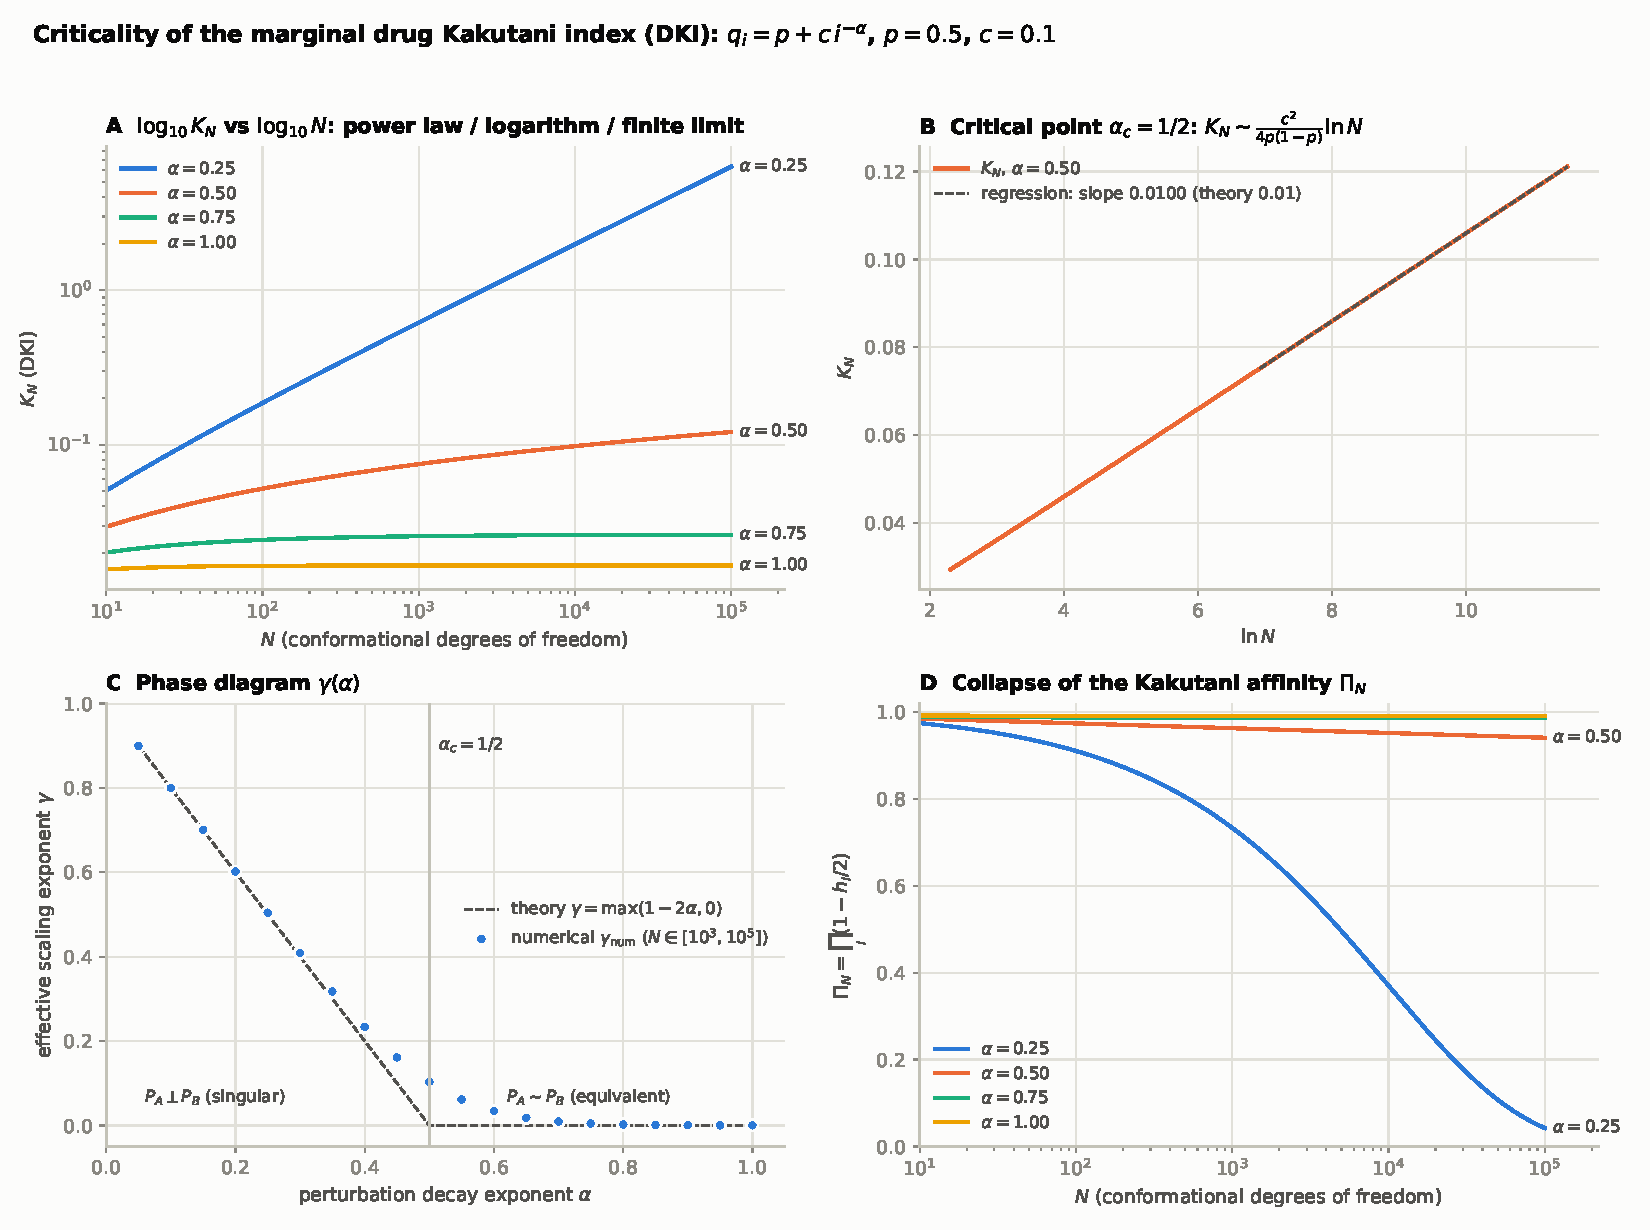
\includegraphics[width=\textwidth]{fig01_marginal_dki_phase_transition.pdf}
\caption{Criticality of the marginal drug Kakutani index for $q_i=\frac12+\frac1{10}i^{-\alpha}$ (\texttt{figures/fig01\_marginal\_dki\_phase\_transition.pdf}, with a PNG copy alongside).
\textbf{A.} $K_N$ against $N$ on doubly logarithmic axes for $\alpha=0.25,0.5,0.75,1$. The supercritical curve ($\alpha=0.25$) is a straight line of slope $\to\frac12$, the signature of $K_N\sim2A\sqrt N$; the critical curve bends downward continuously, as a logarithm must on these axes; the subcritical curves saturate at the finite limits $K_\infty(0.75)=0.026277$ and $K_\infty(1)=0.016587$ of \eqref{eq:sub}. The vertical order of the curves at fixed $N$ is the order of $H_N(2\alpha)$.
\textbf{B.} $K_N$ against $\ln N$ at $\alpha=\alpha_c$: a straight line of slope $A=0.01$ (regression $0.0099992$), the intercept being $A\gamma_{\mathrm{EM}}+C_\infty(\frac12)=0.005981$; the strict linearity over four decades is the content of \eqref{eq:crit}, and its slope is the Fisher-information prefactor $c^2/(4p(1-p))$.
\textbf{C.} The phase diagram: the measured regression exponent $\gnum(\alpha)$ (points) against the asymptotic $\max(1-2\alpha,0)$ (dashed). The points lie systematically above the line for $\alpha<\frac12$ and approach it from above as $\alpha\to0$; the excess is $\geff-(1-2\alpha)$ of Theorem~\ref{thm:fss}, growing with $|\zeta(2\alpha)|$ as the pole at $2\alpha=1$ is approached, and it does not vanish at $\alpha_c$ but joins continuously to $1/(\ln N+\gamma_{\mathrm{EM}})$ by \eqref{eq:geffcrit}. For $\alpha>\frac12$ the points decay to $0$ as $N^{1-2\alpha}$, the rate of saturation in \eqref{eq:sub}. The vertical line marks the Kakutani boundary: to its left the infinite ensembles are mutually singular, to its right equivalent.
\textbf{D.} The Kakutani affinity $\Pi_N=\prod_{i\le N}(1-h_i/2)$. At $\alpha=0.25$ it collapses to $0.0426$ at $N=10^5$ along $\exp(-K_N/2)$; at $\alpha_c$ it decays as the power $N^{-A/2}=N^{-0.005}$ (from $0.9853$ at $N=10$ to $0.9412$ at $N=10^5$) and will reach zero only logarithmically slowly; at $\alpha=0.75$ and $1$ it has converged, to within $3\times10^{-5}$ and $10^{-7}$ respectively, to its positive limits $\Pi_\infty=0.98693$ and $0.99173$. Every finite-$N$ affinity is strictly positive: the singularity is a statement about the limit, as Theorem~\ref{thm:kakutani} requires.}
\label{fig:phase}
\end{figure}

\subsection*{Reading the tables}
Three features of Table~\ref{tab:bench} deserve comment. First, the agreement between $K_N$ and $K_N^{\mathrm{EM}}$ improves with $N$ as a power, from $10^{-7}$ at $N=10$ (the neglected $O(N^{-s-3})$ term of \eqref{eq:EMs}) to $10^{-10}$--$10^{-13}$ at $N=10^5$, in accordance with the asymptotic character of the Euler--Maclaurin expansion; the data are exact to double precision, and the residual at large $N$ is rounding. Second, the column $\Dtail(N)$ separates the three phases without any fit: it grows as $N^{1/2}$ at $\alpha=0.25$ (ratio $\approx3.16$ per decade), converges to $0.00693$ at $\alpha_c$, and decays as $N^{-1/2}$ resp.\ $N^{-1}$ at $\alpha=0.75$ resp.\ $1$ (ratios $\approx0.316$ and $0.1$ per decade). Third, $\Pi_N$ at $N=10^5$ equals $0.9412$ at the critical point and $0.9870$ in the nearest subcritical case: no finite-$N$ observable distinguishes ``will collapse to zero'' from ``has converged to $0.987$'' by its value alone---only the scaling with $N$ does, which is why $\Dtail$ and not $\Pi_N$ is the diagnostic proposed here. Table~\ref{tab:scaling} shows that the pole-corrected exponent $\gEM^{\mathrm{fit}}$ predicts $\gnum$ to within $3\times10^{-4}$ over the whole range, and that $\gtail$ is unbiased to within $5\times10^{-4}$.

%%%%%%%%%%%%%%%%%%%%%%%%%%%%%%%%%%%%%%%%%%%%%%%%%%%%%%%%%%%%%%%%%%%%%%%%%%%%%%%
\clearpage
\section{Assessment and bridge to Paper II}
\label{sec:assessment}

We separate what is established from what is not.

\subsection*{Established unconditionally}
Within the product model of Definition~\ref{def:ensemble}: the product formula and the logarithmic sandwich for the affinity (Lemma~\ref{lem:affinity}); the exact quartic expansion \eqref{eq:taylor} and the even closed form \eqref{eq:half} at $p=\frac12$ (Lemma~\ref{lem:taylor}); the trichotomy with its constants (Theorem~\ref{thm:trichotomy}), the critical doubling identity (Proposition~\ref{prop:doubling}), the effective-exponent law \eqref{eq:geff} with its continuity \eqref{eq:geffcrit} through the critical point (Theorem~\ref{thm:fss}), and the unbiasedness of the doubling estimator (Corollary~\ref{cor:tail}). The numerical benchmarks of Section~\ref{sec:numerics} are consistent with these statements to the precision of double arithmetic; they verify the theorems, they are not needed for them.

\subsection*{Conditional or incomplete}
The identification of the physical ensemble with a \emph{product} measure is a modelling assumption, and it is the one that Paper~II removes. The power law $q_i=p+ci^{-\alpha}$ is a model of allosteric decay along a one-dimensional index; a residue graph with its own metric would replace $i^{-\alpha}$ by a decay in graph distance and $H_N(2\alpha)$ by a growth function of the graph, and the trichotomy would be inherited from the growth rate of that function. The critical value $\alpha_c=\frac12$ is therefore specific to $\mathbb Z$-like indexing; what is model-independent is the mechanism (square-summability of the local Hellinger coordinates) and the diagnostic (the doubling tail). Finally, $N\to\infty$ is an idealisation: a protein has finitely many residues, and Lemma~\ref{lem:affinity} shows that every $\Pi_N$ is strictly positive. The theorems say how the finite-$N$ observables scale, and Section~\ref{sec:fss} shows that the scaling, not the value, is what can be read off.

\subsection*{Relation to the literature}
Kakutani's theorem \cite{Kakutani1948} and its Gaussian form \cite{Feldman1958,Hajek1958} are classical; the Hellinger affinity and its relation to Fisher information are in \cite{Hellinger1909,Bhattacharyya1943,LeCam1986}. The transport from \cite{Chen2026} is at the level of the criterion (the dictionary of \S\ref{sec:intro}); nothing here uses the operator-algebraic structure of the Bost--Connes system, and conversely nothing there uses the Bernoulli structure. The ensemble view of allostery \cite{Motlagh2014,Nussinov2013} supplies the physical premise that function is a property of the joint distribution; we have not seen the Kakutani dichotomy used in that literature, and a literature check remains advisable.

\begin{table}[ht]
\centering\small
\caption{Assessment of Paper I.}
\label{tab:assessment}
\begin{tabular}{@{}p{0.46\textwidth}p{0.2\textwidth}p{0.26\textwidth}@{}}
\toprule
Item & Status & Where \\
\midrule
DKI, affinity, doubling tail; product formula $\Pi_N=\prod(1-h_i/2)$ & established & Def.~\ref{def:dki}, Lemma~\ref{lem:affinity} \\
Quartic expansion of $h$; vanishing of odd terms and closed form at $p=\frac12$ & established & Lemma~\ref{lem:taylor} \\
Phase trichotomy, $\alpha_c=\frac12$, constants $A\zeta(2\alpha)$, $C_\infty(\alpha)$ & established (product model) & Thm.~\ref{thm:trichotomy} \\
Critical doubling constant $A\ln2$ & established & Prop.~\ref{prop:doubling} \\
Effective exponent $\geff(N;\alpha)$; near-critical bias $=$ pole of $\zeta$ & established & Thm.~\ref{thm:fss}, Rem.~\ref{rem:045} \\
Unbiased doubling estimator & established & Cor.~\ref{cor:tail} \\
Benchmarks at $N=10^5$; agreement with Euler--Maclaurin to $10^{-10}$ & verified numerically & Tables~\ref{tab:bench}, \ref{tab:scaling} \\
Independence of local switches & modelling assumption & \S\ref{sec:assessment}, Paper II \\
Identification of $\alpha$ with a structural decay length & open & Problem (2) \\
Covariance-driven transition with all marginals fixed & open & Problem (1), Paper II \\
\bottomrule
\end{tabular}
\end{table}

\subsection*{Open problems and the bridge to Paper II}
\begin{enumerate}[label=(\arabic*),leftmargin=*]
\item \emph{Covariance dominance.} Residue fluctuations in a real protein are not independent: hydrogen-bond networks, disulfide bridges and the hydrophobic core couple them through a covariance matrix $C_{ij}$. Consider the Gaussian ensembles $\mathcal N(\mu_A,C_A)$ and $\mathcal N(\mu_B,C_B)$ on $\Rr^N$, for which the Bhattacharyya distance $D_B=D_{\mathrm{mean}}+D_{\mathrm{cov}}$ splits into a mean part, which is the continuous analogue of the DKI studied here, and a covariance part
\[
D_{\mathrm{cov}}=\frac12\ln\frac{\det\frac12(C_A+C_B)}{\sqrt{\det C_A\det C_B}} .
\]
Suppose the mean shifts $\Delta\mu_i$ lie in the subcritical regime of Theorem~\ref{thm:trichotomy}---or vanish identically, $\Delta\mu_i\equiv0$ and $\Delta\mathrm{RMSF}_i\equiv0$, so that the marginal index is $K_N\equiv0$. Can the off-diagonal re-arrangement of $C_{ij}$ alone drive the Feldman--H\'ajek dichotomy into the singular regime, i.e.\ $D_{\mathrm{cov}}\to\infty$ as $N\to\infty$? The finite-dimensional Gaussian measures are always equivalent, so the question is one of scaling of $D_{\mathrm{cov}}$ with $N$, and the doubling-tail diagnostic of Corollary~\ref{cor:tail} applies verbatim. Paper~II defines the correlated Kakutani index (CKI) and examines the regime---suggested by preliminary computation and to be established there---in which the covariance term carries the overwhelming share of $D_B$ while every marginal is unchanged.
\item \emph{What is $\alpha$?} Relate the decay exponent to a measurable property of the residue-interaction graph (its growth function or spectral dimension), so that $\alpha\lessgtr\alpha_c$ becomes a structural prediction rather than a fitted parameter.
\item \emph{Beyond $p=\frac12$.} For $p\ne\frac12$ the cubic term of \eqref{eq:taylor} does not vanish and the sign of $\delta_i$ matters; the trichotomy persists (the quadratic term still dominates) but the constants acquire odd contributions $\propto c^3H_N(3\alpha)$. Determine whether the maximal-entropy point $p=\frac12$ is selected physically by the ground state or is merely convenient.
\item \emph{The arithmetic side.} The dictionary of \S\ref{sec:intro} suggests that the finite-size theory of Section~\ref{sec:fss}---the pole of $\zeta$ as the source of apparent exponents---has a counterpart for the obstruction group $\Xi_\beta(K,S)$ of \cite{Chen2026} when $S$ is a finite truncation of an infinite set; whether the ``doubling'' estimator has an arithmetic meaning is not known to us.
\end{enumerate}

\subsection*{Reproducibility}
\begin{sloppypar}
All results are generated by \texttt{code/exp01\_marginal\_dki\_criticality.py} (data, figure, acceptance tests) and \texttt{code/paper01\_compute\_tables.py} (analytic constants, Tables~\ref{tab:bench}--\ref{tab:scaling}); both run in seconds with NumPy, Matplotlib and mpmath. The paper and its \LaTeX{} source (\texttt{paper/}), the raw data (\texttt{data/}), the figure (\texttt{figures/}) and the derived tables (\texttt{results/}) are archived under DOI \href{https://doi.org/10.5281/zenodo.23005921}{10.5281/zenodo.23005921} and maintained in the repository \texttt{kakutani-statistical-pharmacology-I}.
\end{sloppypar}

\subsection*{Funding}
This project was supported by the National Natural Science Foundation of China (No.~22464010), the Guangxi Natural Science Foundation of China (No.~2025GXNSFAA069294), and the 2025 Bagui Youth Top Talent Project.

\begin{thebibliography}{99}
\bibitem{Apostol1999} T.~M. Apostol, \emph{An elementary view of Euler's summation formula}, Amer. Math. Monthly \textbf{106} (1999), 409--418.
\bibitem{Bhattacharyya1943} A.~Bhattacharyya, \emph{On a measure of divergence between two statistical populations defined by their probability distributions}, Bull. Calcutta Math. Soc. \textbf{35} (1943), 99--109.
\bibitem{BostConnes1995} J.-B. Bost and A.~Connes, \emph{Hecke algebras, type III factors and phase transitions with spontaneous symmetry breaking in number theory}, Selecta Math. (N.S.) \textbf{1} (1995), 411--457.
\bibitem{Chen2026} R.~Chen, \emph{Localized Bost--Connes systems}, assembled from the thirty-nine papers of the series, 2026, DOI 10.5281/zenodo.22883179.
\bibitem{Feldman1958} J.~Feldman, \emph{Equivalence and perpendicularity of Gaussian processes}, Pacific J. Math. \textbf{8} (1958), 699--708.
\bibitem{Hajek1958} J.~H\'ajek, \emph{On a property of normal distributions of any stochastic process}, Czechoslovak Math. J. \textbf{8} (1958), 610--618.
\bibitem{Hellinger1909} E.~Hellinger, \emph{Neue Begr\"undung der Theorie quadratischer Formen von unendlichvielen Ver\"anderlichen}, J. Reine Angew. Math. \textbf{136} (1909), 210--271.
\bibitem{Kakutani1948} S.~Kakutani, \emph{On equivalence of infinite product measures}, Ann. of Math. (2) \textbf{49} (1948), 214--224.
\bibitem{LeCam1986} L.~Le~Cam, \emph{Asymptotic Methods in Statistical Decision Theory}, Springer, New York, 1986.
\bibitem{MWC1965} J.~Monod, J.~Wyman and J.-P. Changeux, \emph{On the nature of allosteric transitions: a plausible model}, J. Mol. Biol. \textbf{12} (1965), 88--118.
\bibitem{Motlagh2014} H.~N. Motlagh, J.~O. Wrabl, J.~Li and V.~J. Hilser, \emph{The ensemble nature of allostery}, Nature \textbf{508} (2014), 331--339.
\bibitem{Nussinov2013} R.~Nussinov and C.-J. Tsai, \emph{Allostery in disease and in drug discovery}, Cell \textbf{153} (2013), 293--305.
\bibitem{Titchmarsh1986} E.~C. Titchmarsh, \emph{The Theory of the Riemann Zeta-Function}, 2nd ed., revised by D.~R. Heath-Brown, Oxford University Press, 1986.
\end{thebibliography}

\end{document}
